\chapter{Autonomous System}
\label{ch:Autonomous_System}
The autonomous software design of a passenger aircraft faces many challenges, from accuracy and reliability to public acceptance.
Being a new technology, the introduction of such a system shall be gradual.
Firstly, a fully autonomous flight with emergency local manual control may be introduced.
Then fully autonomous systems can be employed with remote safety control in case of emergency until fully autonomous flights are not completely reliable.
The following chapter walks the reader through the conceptual design of the autonomous system of the \textit{Swing} UAM. Firstly, the necessary functions of the system are investigated.
Subsequently, the description of the software architecture and control modes are presented.
Eventually, the critical sensors are collected to estimate the full dynamic state of the UAM.

\section{Autonomous Software Functions}
Before the conceptual design of the autonomous software, the necessary functions of such software must be summarized.
Firstly, it has to find an obstacle-free path between the starting location and the destination.
Meanwhile, a communication link shall be created between the vehicle and the ground control.
The aircraft's steering is done with several different controllers in different flight conditions through the actuators.
Finally, several diagnostic algorithms shall be implemented to ensure the safety of the passengers and the surroundings.

As mentioned before, the steering input of the UAM is calculated by different control modes.
The following control modes are identified by inspecting the mission profile presented in \Cref{fig:mission_profile}.
The UAM has to perform a vertical take-off and landing in a hexacopter configuration alongside hovering.
Next, the vehicle performs a forward and backward transition with complex dynamics requiring a different controller.
Whilst, the fixed-wing configuration shall perform a climb, cruise and descent.
The last three modes having similar dynamics are controllers with the same control mode.
Lastly, a remote manual control mode is required to take safety measures.
In the following section, these control modes are further elaborated, and an appropriate control architecture is selected for each.

\section{Autonomous Software Architecture}
The following section aims to present the conceptual design of the autonomous controller.
To facilitate an easy understanding of the subcomponents of the design, first, the reader is provided with an overview of the structure and flow of the autonomous software.
\Cref{fig:autonomous_software_diagram} summarises the most important components and actions within the software.

The system's start-up triggers a diagnostic software ensuring the safe start of the flight and compliance with requirements Te-1-STK04-3 and Te-1-STK04-3-1.
If this process runs into issues, the system blocks the possibility of flight, guaranteeing the safety of the passengers.
Otherwise, the flight can commence by communicating with the air traffic database and starting the route planning block.
The route planning algorithm ensures that the most efficient obstacle-free route is found whilst air traffic regulations and separation standards are met utilising the air traffic and sensor data.
Here, an iterative process can be found between the air traffic centre and the local vehicle, as the aim of the algorithm is not just to find an optimal route for a single agent but for all agents.
Subsequently, if the route planner executes without an error, the control mode of the aircraft is selected, then the eVTOL controller can start the operation in a closed loop.
Due to the longer running time of the global route planner algorithm, the control loop is called with a higher frequency than the global route planner algorithm.
If an issue is detected within the planner loop, the air traffic controller is alarmed, who will attempt to resolve the issue.
In case the issue cannot be solved, the command of the aircraft is transferred to a remote manual pilot who safely navigates the UAM to the destination.
In the event of flawless operation, the autonomous software ensures a smooth flight and reaches the destination in the shortest possible time.

In the following subsections, some of the software blocks are further detailed.
Firstly, the conceptual design of the route planner algorithm is presented.
Next, the control strategy is selected for different control modes alongside the conceptual design of the controllers.
Lastly, recommendations are made for future work to complete the design and implementation of the autonomous software.
\begin{figure}[ht]
    \centering
    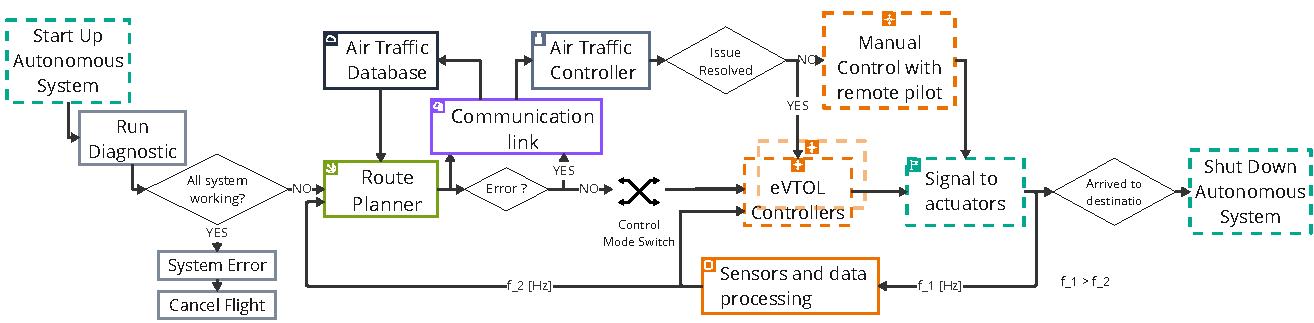
\includegraphics[width=\linewidth]{figures/autonomous/autonomous_software_diagram}
    \caption{Flow diagram of the autonomous software}
    \label{fig:autonomous_software_diagram}
\end{figure}

\subsection{Global Route Planner}
As proposed before, the global route planner holds the most importance in the autonomous software structure.
This algorithm ensures that the vehicle arrives from the start location to the desired destination without any accidents.
The highest level goal of this algorithm is to find a path between set waypoints (and potentially return to the starting point) without collision, minimising a pre-defined cost function.
This route-finding problem is essentially a Travelling Salesman Problem (TSP), for which several approximate algorithms exist.
Firstly, the existing algorithms for this problem are compared.
After selecting the most suitable one, the final structure of the planner is presented.

 For discrete path planning and obstacle avoidance, two widely used algorithms exist, the Probabilistic RoadMaps (PRM) and the Rapidly Exploring Random Trees (RRT) \cite{PRM,RRT}.
  Furthermore, several derivative algorithms exist and are proposed.
    In order to select the most suitable algorithm, a simple comparison is performed.
        Starting with the RRT algorithm, asymptotic stability is not ensured, meaning it does not approach the optimal route by increasing the spatial sample number.
                On the other hand, the simple PRM (sPRM) variant of the PRM method is proven to be asymptotically optimal.
                                Contrary, the time complexity of the RRT ($\operatorname{O}(n\log n$) algorithm over-performs the one of sPRM ($\operatorname{O}(n^2)$) \cite{prm_rrt}.
  Since no other major advantage difference can be detected between the two algorithms, a trade-off has to be made based on the more desired property.
    As the profit is indirectly influenced by the flight time, it is desirable to obtain the optimal root over the decreased computational capacity.
        This possibly results in an increased flight number capacity over a fixed time, implying an increased profit.
                Furthermore, if necessary, this process can be performed on a remote computer instead of the on-board computer allowing for faster computation.
                                Therefore, the PRM algorithm was selected.

The PRM algorithm requires several subcomponents to operate, including point sampling, obstacle-checking and shortest-path algorithms.
Roland G. et al.\ compare several sampling techniques for PRM planners \cite{sampling}.
Since no straightforward conclusion can be drawn from the study, the paper can later help to select the most appropriate technique for the case of urban air mobility.
To meet requirement Co-6-STK12, the point cloud must be generated such that the air traffic regulations are met.

The next challenge of discrete path planning is the obstacle-checking algorithm.
This algorithm must take into account the fixed and moving obstacles obtained from city maps and from the flight operator alongside the local obstacles detected by the radar and computer vision system.
To speed up the collision checking, a safety certificate method was introduced by Joshua B. et al.
can be implemented \cite{safety_certificates}.
This process generates spherical safety certificates around the sample points.
Consequently, the computational time required for obstacle-checking decreases exponentially with increasing certificate numbers since obstacle-checking with spheres is less computationally demanding.
It is important to note that a safety margin of three meters plus the sensors’ uncertainty must be considered when the radii of the safety certificates are calculated.
Hence, the violation of requirement Co-5-STK14-2-2, which requires a three-meter safety margin between any object and the vehicle, is avoided.
Furthermore, to satisfy requirement Co-6-STK12, the air traffic regulations and separation standards must be met when the obstacle checking is done \cite{multy_agent_ATC1}.

For path finding an A-star algorithm is proposed due to its optimality and fast computational time.
However, the optimality requires an admissible heuristic, meaning that the estimated cost-to-reach must underestimate the real cost-to-reach.
The proper design of the cost function and heuristic will be performed in the later stages of the design; however, it is important to note that the route has to cover the most amount of distance in the shortest time with the least amount of electricity possible.
The final component of this algorithm is to fit a Dubins’ tour on the achieved points, ensuring the fastest continuous path that can be fit on the discrete route \cite{dubins}.

The previous considerations only accounted for a single-agent system.
However,
it is important to emphasise that this problem contains several agents in the form of other UAMs and possibly UAVs.
Therefore, to ensure global optimality and account for uncertainties,
the problem must be solved as a multi-agent problem.
Paul O. et al.
proposed a transformation between a multi-agent TSP  and an asymmetric TSP which can subsequently be solved with any routing algorithm \cite{todays_traveling_salesman}.

These considerations guarantee that all the necessary components are present for a global route planner.
The algorithm’s essential parts and flow are shown on \Cref{fig:route_planner_diagram}.

\begin{figure}[H]
    \centering
    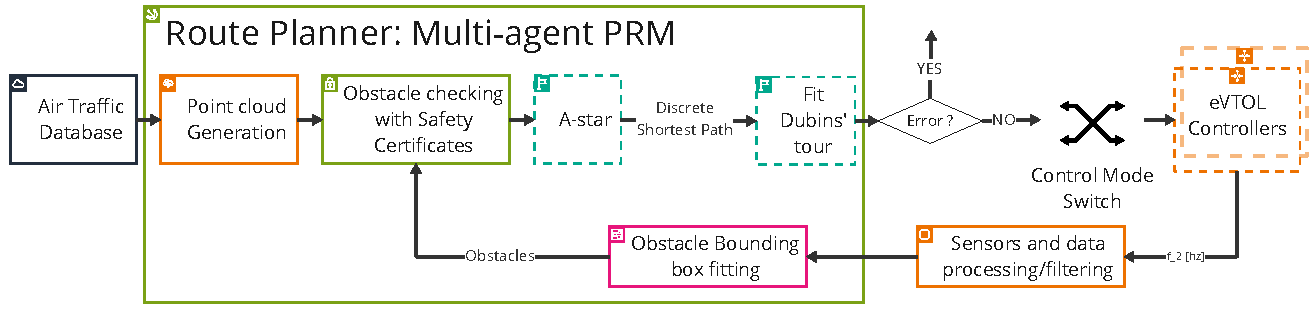
\includegraphics[width=\linewidth]{figures/autonomous/route_planner_diagram}
    \caption{Flow diagram of route planning software}
    \label{fig:route_planner_diagram}
\end{figure}

\subsection{Hexacopter Control: Vertical Take-off, Landing and Hovering modes}
The aim of the vertical take-off and landing control mode is to reach a specified altitude while maintaining the same position in the other two dimensions.
Similarly, the purpose of the hovering control is to sustain a fixed position in the space.
Hence, the same controller architecture was selected for both conditions.
As the vehicle spends a short time in these configurations, a simple but reliable control structure is needed.
Thus, the position control architecture depicted in \Cref{fig:hexacopter_diagram} is selected for position control.

The structure contains three separate PID controllers to successfully achieve active control over the hexacopter configuration.
Firstly, three separate PD controllers estimate the necessary thrust vector compensation in the inertial frame.
Subsequently, using a coordinate transformation between the inertial frame and the body frame, the desired pitch ($\Theta$) and roll ($\Phi$) angles are calculated and controlled to perform the attitude control of the vehicle.
The PD attitude controllers calculate the virtual control inputs of thrust ($U_1$) and moments about the $x$, $y$ and $z$ axes ($U_2, U_3, U_4$), which can be transformed to the angular speeds of the motors by solving \Cref{eq:alloc_mx}.
Here, $b$ and $d$ are the lift and drag coefficients of the rotors, $x_i, y_i$ are the moment arms from the centre of gravity, whilst $n_i$ takes a value of $1$ if the rotor is rotating clockwise, else $-1$.
Since for the allocation matrix $n < m$, infinitely many solutions exist.
Thus, if R is full row rank, the right pseudo inverse of R can be taken to minimise the control effort as shown in \Cref{eq:alloc_mx} \cite{quadcopter_control_allocation}.
Finally, the motor speed PID controllers sustain a stable rpm by controlling the current or potential on the actuators.
\begin{align}
\label{eq:alloc_mx}
    &\underbrace{\begin{bmatrix}
        U_1\\U_2\\ U_3\\U_4
    \end{bmatrix}}_{\text{U}} = 
    \underbrace{\begin{bmatrix}
        b & b & b & b & b & b \\
        by_1 & by_2 & by_3 & by_4 & by_5 & by_6 \\
        bx_1 & bx_2 & bx_3 & bx_4 & bx_5 & bx_6 \\
        dn_1 & dn_2 & dn_3 & dn_4 & dn_5& dn_6
    \end{bmatrix}}_{\text{R}^{n\times m}} \ 
    \underbrace{\begin{bmatrix}
        \omega^2_1\\
        \omega^2_2\\
        \omega^2_3\\
        \omega^2_4\\
        \omega^2_5\\
        \omega^2_6
    \end{bmatrix}}_{\Omega} & & & \Omega = \text{R}(\text{R}^\text{T}\text{R})^{-1}\text{U}
\end{align}

\begin{figure}[H]
    \centering
    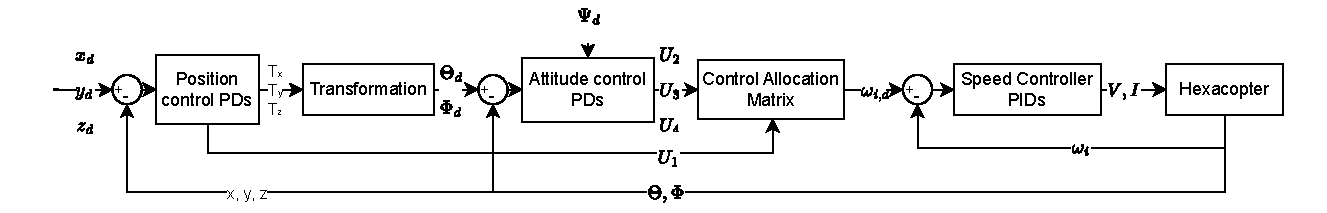
\includegraphics[width=\linewidth]{figures/autonomous/hexacopter_diagram}
    \caption{Position control loop for vertical take-off, landing and hover}
    \label{fig:hexacopter_diagram}
\end{figure}

In the extreme case of two frontal engine failures or the failure of more than three engines, the stabilisation and safe landing shall be ensured in hexacopter configuration.
Mark W. et al.
proposed a fault-tolerant multicopter controller which is capable of stabilising the vehicle in case of multiple engine failures by sacrificing the yaw control and thus passenger comfort \cite{fault_tolerant}.
Furthermore, if no precise state estimation is available through external sensors (GPS), the onboard computer vision can be utilised to measure the state of the vehicle \cite{fault_tolerant_compvis}.

\subsection{Transition Mode}
The transition control was realised utilising a combination of three controllers similarly as shown in \cite{transition_control}.
A planar altitude controller provides stable altitude tracking, whilst an attitude controller ensures precise altitude stabilisation.
Finally, a torque ($\tau$) controller regulates the angular rate of the transition mechanism.

However, due to the highly nonlinear nature of the process, the gains of the controller cannot be optimised for all flight conditions.
This issue can be resolved by employing a gain-scheduling controller.
The nonlinear model can be linearised around pre-specified transition angle values ($q$), and the controller gains can be tuned for each working point achieving great performance \cite{gain_scheduling}.
The proposed controller is summarised in the block diagram of \Cref{fig:transition_diagram}.
Here the actuator controller has a simple mass spring damper structure with an added estimate gravity term to eliminate the steady state error as shown in \Cref{eq:mass_spring_damper}.
The gravity term can be calculated using the positional Jacobian between the centre of gravity and inertial frame as shown in \Cref{eq:mass_spring_damper}.
The precise design of the terms in the attitude and altitude controllers opted to be done after the precise dynamic simulation of the transition is done.

%It is selected that the forward and backward transition is controlled by a %linear gain scheduling control. This decision was made on the simplicity and %robustness of the controller. Furthermore, it is proven by\cite{} that a %small-scale version of a similar transitional vehicle can be controlled by %such controller. To elaborate more on the controller design a Linear %Parameter Varying (LPV) Linear Quadratic Regulator (LQR) controller is %selected as proposed in \cite{}. As a first step, the nonlinear modelling of %the transition has to be done. 

\begin{figure}[h!]
    \centering
    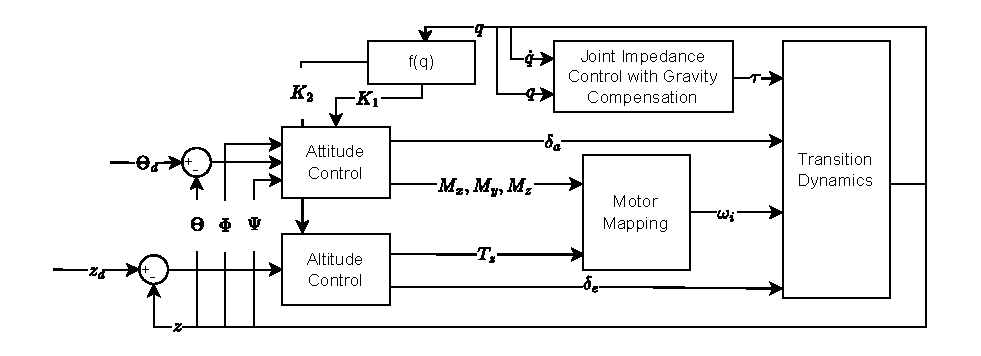
\includegraphics[width=\linewidth]{figures/autonomous/transition_diagram}
    \caption{Transition control loop with attitude, altitude tracker and joint impedance controller with gravity compensation}
    \label{fig:transition_diagram}
\end{figure}
\begin{align}
\label{eq:mass_spring_damper}
    \tau_d &= k_p(q_d-q) + k_d(\dot{q}_d-\dot{q}) + \hat{g}(q) & & \hat{g}(q) = \sum_{i=1}^{2} - _I J_{P_i} \cdot _I F_{g, i}
    \end{align}
\subsection{Fixed Wing Control: Cruise, Climb and Descent Modes}
The control mode possessing the most importance is the cruise controller since it is the control mode in which the aircraft spends the most amount of time.
The fully autonomous passenger flight area is a developing field; therefore, no controller type has gained the trust of the engineers in this field.
Thus, a simple comparison is performed on the most common controller types, LQR, PID and Model Predictive Control (MPC) to select the most suitable one.

In a disturbance-free environment, PID and LQR controllers outperform the tracking capabilities of MPC controllers.
However, in cases where disturbance rejection of the controller is highly important, which is the case during cruising, MPC controllers show a better performance.
In the case of the transwing eVTOL vehicle, the property of disturbance, and therefore wind, rejection is of utmost interest due to the requirement of Te-2-STK07-5-2.
Furthermore, generally speaking, the control effort is much less in the case of MPC compensators compared to its opponents \cite{MPC_justification}.
Additionally, the robustness of MPC controllers cannot be overlooked as it is important to achieve high accuracy in a wide range of weather and environmental conditions.

As an optimal control problem, MPC enables achieving high performance in the desired performance metrics.
The availability of setting control contains can enable smooth changes between states, thus avoiding high accelerations resulting in higher passenger comfort and complying with requirements Te-2-STK07 and Te-2-STK07-1-4.
Lastly, with this control scheme, it is possible to incorporate local obstacle avoidance with obstacle convexification proposed by \cite{convexification}.
The aforementioned list of advantages of MPC gives confidence that the best choice for cruise control is an MPC compensator.

Since the main objective of the aircraft mission is to reach the destination in the shortest time, a Model Predictive Contouring Controller (MPCC) was selected as the optimisation problem.
This controller shows superior performance over conventional state trajectory tracking MPC controllers by minimizing the contouring and lag errors with respect to a pre-defined reference path described by a cubic spline \cite{MPCC}.
The optimisation problem is formulated as shown by Equations \ref{eq:MPCC_opt}-\ref{eqn:approx_dynamics}.
Here the linearised contouring error ($\hat{e}^\mathrm{c}$) and the lag error ($\hat{e}^\mathrm{l}$) are the transverse and lateral distances between the current position ($p_k$) and the estimated position on the reference path as depicted in \Cref{fig:MPCC_errors}.
The parameter $v_k^{\hat{\theta}}$ is the virtual tracking speed on the reference trajectory and $q_c$, $q_l$, $\gamma$ are weights for the cost terms.
Potentially, a cost term can be added to this optimisation statement that minimises energy consumption, whilst it shall be extended with the necessary constraints for obstacle avoidance as shown in \cite{convexification}.

\begin{minipage}{.4\textwidth}
        \begin{figure}[H]
        \centering
        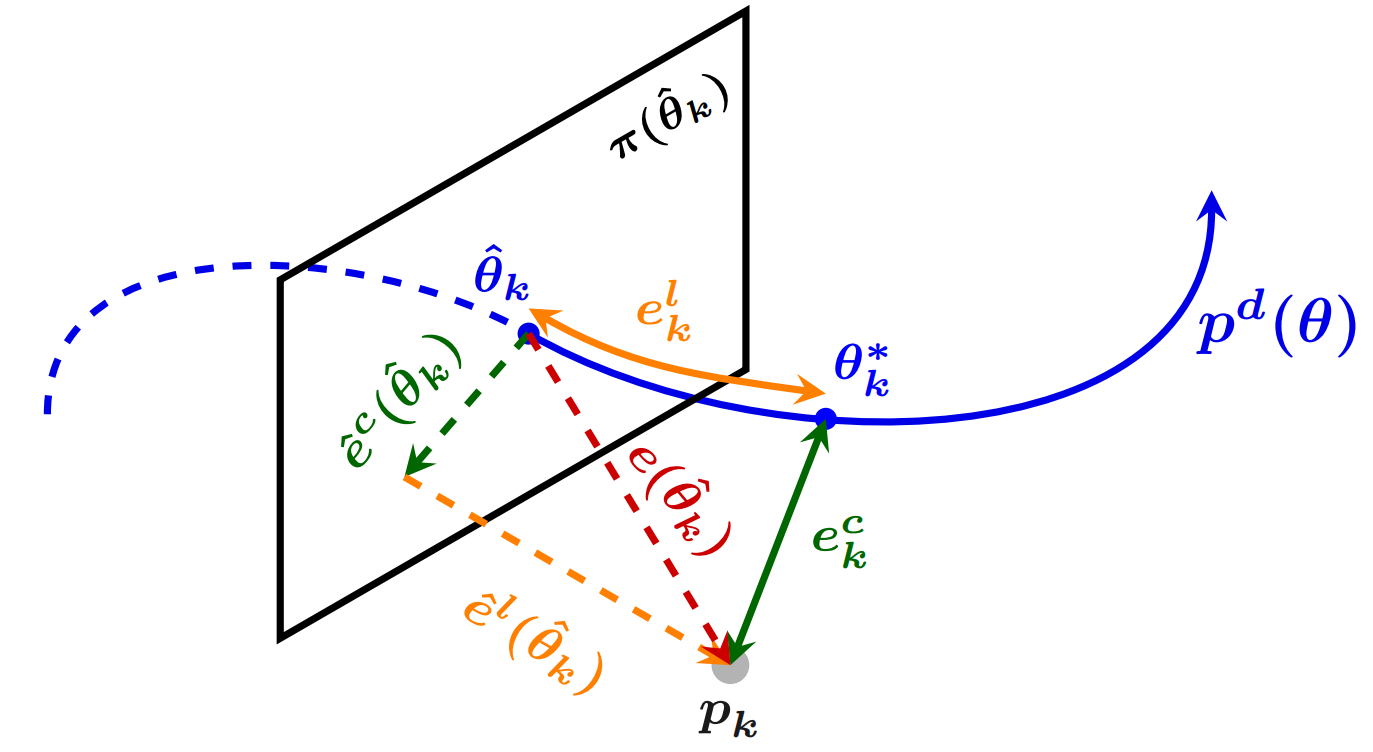
\includegraphics[width=\linewidth]{figures/autonomous/errors}
        \caption{Contouring and lag error defined for the MPCC controller \cite{MPCC}}
        \label{fig:MPCC_errors}
\end{figure}
    \end{minipage}%
    \begin{minipage}{0.6\textwidth}
        \centering
        \begin{align}
        \label{eq:MPCC_opt}
        \min_{x, u, v}  \quad & \sum_{k=1}^N \lVert \hat{e}^\mathrm{c}(x_k,y_k,z_k,\hat{\theta}_k) \rVert_{q_\mathrm{c}}^2+\lVert \hat{e}^\mathrm{l}(x_k,y_k,z_k,\hat{\theta}_k) \rVert_{q_\mathrm{l}}^2-\gamma v^{\hat{\theta}}_k\\
        \text{subject to} \quad & \mathpzc{x}_0=\mathpzc{x},\\
                            \label{eqn:disc_model_opt}
                            \quad & \mathpzc{x}_{k+1}=f(\mathpzc{x}_k,u_k),\qquad k=1,\dots,N-1,\\
                            \quad &  \mathpzc{x}_k\in\mathcal{X}, u_k\in\mathcal{U}, \Delta\mathpzc{x}_k\in\Delta\mathcal{X}, \Delta u_k\in\Delta\mathcal{ U},\\
                            \quad & \hat{\theta}_0=\theta,\\
                            \label{eqn:approx_dynamics}
                            \quad & \hat{\theta}_{k+1}=\theta_k+v^{\hat{\theta}}_k\Delta t,
        \end{align}
    \end{minipage}

\Cref{eqn:disc_model_opt} uses a nonlinear dynamic function to predict the states of the cruising UAM.
Hence, optimisation can only be solved as a nonlinear program (NP).
The current state-of-the-art NP solvers, such as IPOPT, implement the interior point primal-dual method.
This method does not guarantee global optimality, what is more, convergence is not ensured to local minima in acceptable time \cite{IPOPT}.
Therefore, it is recommended to linearise the cruise dynamics about different working points,
generating a Linear Parameter Varying (LPV) model enabling the solving of the problem with a Quadratic Program
(QP).
One form of such a model is shown by \Cref{eqn:lpv_form},
where A and B are the state matrices dependent on the scheduling variables of $x$ and $u$.
\Cref{eq:lpv_embedding} shows a flexible and easy method to perform the linearisation of the nonlinear dynamics
and constructs the state matrices proposed by \cite{lpv_embedding}.
A necessary requirement of LPV embedding is a nonlinear state derivative at the origin, as shown in \Cref{eq:lpv_condition}.
\begin{align}
    &\dot{x} = f(x, u) && f(0) = 0 \label{eq:lpv_condition}\\
    &A(x, u) = \int_0^1 \frac{\partial}{\partial x}f(\lambda x, \lambda u) \ d\lambda && B(x, u) = \int_0^1 \frac{\partial}{\partial u}f(\lambda x, \lambda u) \ d\lambda \label{eq:lpv_embedding}\\
    &\dot{x} = A(x,u)x + B(x,u)u \label{eqn:lpv_form}
\end{align}
After deriving the nonlinear cruise model of the vehicle, this controller can be easily implemented using a symbolic program package such as CasAdi.
Furthermore, the optimisation problem, being convexified, can be solved with a QP solver.
Furthermore, since a typical control update frequency of such local planners is at the magnitude of a few tens of milliseconds \cite{MPCC}, it might be necessary to speed up the runtime of the algorithm.
If further update time decrease is needed,
an alternative approach to the LPV model is the application of Multiple Shooting Sequential Quadratic Programming, the nonlinear problem.
This method exchanges optimality with computational time decrease with high efficiency as described in \cite{SQP}.
The block diagram of this controller is depicted in \Cref{fig:cruise_diagram}.

\begin{figure}[htpb]
    \centering
    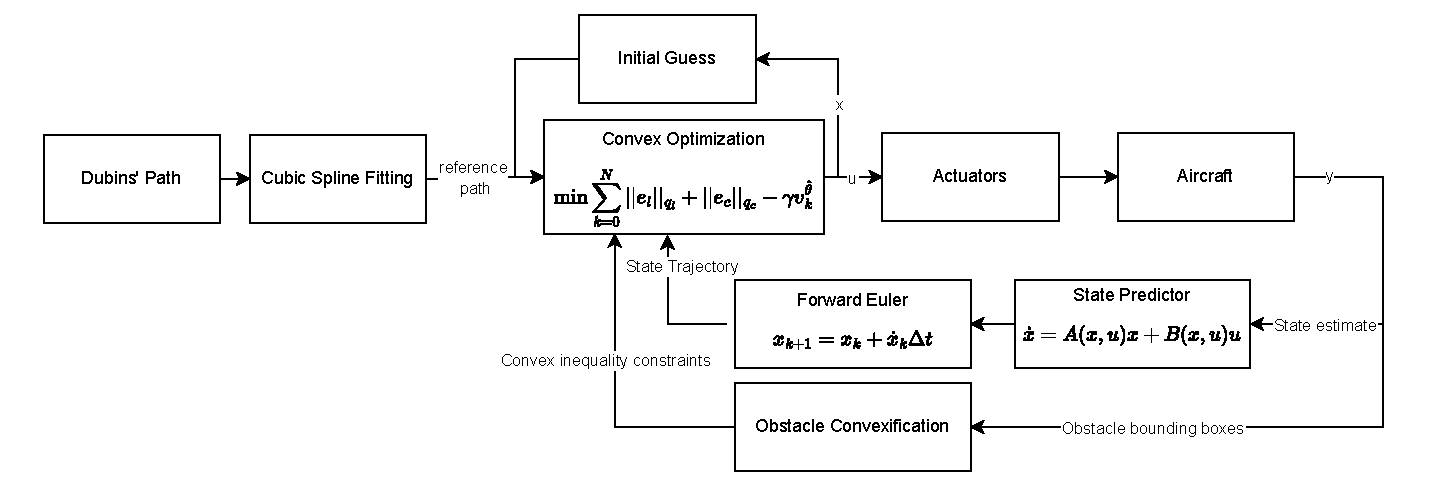
\includegraphics[width=\linewidth]{figures/autonomous/cruise_diagram}
    \caption{MPCC control loop for cruising}
    \label{fig:cruise_diagram}
\end{figure}

Finally, the requirement of Co-3-STK03-1 shall be considered for this control mode.
It demands operation in the case of two inoperative engines.
In \Cref{ch:Stability_and_Control}, it was ensured that it is possible to control and keep the vehicle in the air in the case of two engine failures.
Now the task of the autonomous software is to recognise and adapt to the changes in the system.
Here, another advantage of MPC controllers appears, since after identifying the failed engines, the control system can simply add two new constraints to the optimisation problem of \Cref{eq:MPCC_opt}.
These new constraints ensure that the control inputs corresponding to the failed engines remain zero, allowing for accurate modelling of the system even after engine failures.

\subsection{Future Work}
In the previous sections, several different control methods were proposed.
However, multiple additional steps have to be taken to produce a completely functional autonomous system.
The following, section aims to provide insight into how the future development of this system will proceed.

Firstly and most importantly, the dynamic modelling of the different flight phases has to be done.
In \Cref{sec:Dynamic_Stability_during_Cruise}, a linear model for the cruise phase was proposed.
To further enhance model accuracy, a more detailed nonlinear model can be derived.
Another key modelling aspect of the autonomous software design is the nonlinear modelling of the transition in both directions.
This is inevitable to perform the preliminary tuning of the gain scheduling controller for transition.
Finally, a simple hexacopter model can be selected to tune the PD controllers of the hexacopter position tracking controllers.

After modelling the aircraft in different flight conditions, the model identification has to start to obtain the model parameters.
A fusion of simulation and experimental techniques can be used to determine the precise values of the model parameters.
If all the models are sufficiently developed, the implementation and tuning of the control algorithms can be commenced.
Finally, the controllers shall be tested on the real system.

\section{Measurement System}
In order to perceive the surroundings of the vehicle with sufficient accuracy in any conditions, great care must be taken to select the right types of sensors needed for the autonomous system.
In the previous stages of the design, a preliminary set of sensors was selected.
Now that a detailed conceptual design of the autonomous software has been done, these sensors are revised to ensure all necessary states can be measured.
The following section walks through all these necessary sensors in a top-down manner, meaning first, the higher-level algorithms are considered, and finally, the lower-level controllers.

Firstly, the route planner algorithm has to be considered, which requires a full spatial location estimation with obstacle detection.
As the eVTOL only operates in outdoor conditions, the GNSS and GPS sensors suffice since, in outdoor applications, it can achieve high accuracies of a few centimetres\footnote{\url{https://www.advancednavigation.com/inertial-navigation-systems/mems-gnss-ins/certus/}}.
Regarding obstacle detection, two approaches can be taken, passive or active depth estimation.
Active computer vision utilises time-of-flight (TOF) sensors which can achieve extremely high accuracies at the expense of price and weight.
Furthermore, these sensors can only measure in one direction at a time, meaning it has to scan the entire space before an image can be constructed.
On the other hand, passive depth estimation uses triangulation of camera images.
This strategy cannot achieve such accuracies as TOF sensors; however, they are much cheaper and more flexible as they can perceive the depth through the entire image simultaneously.
Moreover, techniques, such as structured infrared light, exist to enhance the accuracy of passive methods \cite{structured_light}.

Two more important considerations must be taken before selecting the final sensor.
The requirements Te-2-STK07-5-1 and e-2-STK07-5-3 demand the ability to fly in dark and rainy conditions.
TOF sensors have no problem operating in different illumination levels as they only measure the distance from the object.
On the other hand, structured light cameras are equipped with infrared sensors to perceive the structured infrared light projected by the camera system.
Infrared sensors are perfect for night vision.
Moreover, infrared cameras can perform better than TOF sensors in poor weather conditions, such as in heavy rain \cite{rainy_vision}.
Likewise, since structured light cameras can perform with 8-centimetre accuracy on 4 meters\footnote{\url{https://www.intelrealsense.com/stereo-depth-modules-and-processors/}}, the obstacle avoidance requirement of Co-5-STK14-2-2 can be met; thus TOF sensors are disproportionate.
Additionally, passive computer vision has a limited depth estimation range; thus, the use of a radar system is justified for long-range obstacle detection.

Subsequently, the list of required sensors can be continued with the sensors needed for autonomous controllers.
Since the precise model used for these controllers is not developed, the proposed sensors might change after the detailed controller development.
Alongside the spatial position determination, now, the airspeed, temperature, angular rates and accelerations are required to measure the full state of the aircraft.
For this purpose, as proposed beforehand, pitot tubes, inertial measurement units and thermometers can be used.
Furthermore, some computer vision algorithms can aid in increasing the accuracy of the previously mentioned sensors \cite{fault_tolerant_compvis}.
Further, to measure and regulate the control input of the transition actuator, control surface deflection, propulsion throttle and blade pitch actuator encoders can be used.
Concluding the list of sensors, if lower-level current or voltage controllers are to be used to regulate the torque of the actuators, the system has to be equipped with voltmeters or ammeters.

% %TODO: add table with measured states for the final report
% \todo[inline]{add table with measured states for the final report}